\documentclass[12pt, a4paper]{article}
\usepackage[T1]{fontenc}
\usepackage[utf8]{inputenc}
\usepackage[english,russian]{babel}
\usepackage{amsmath}
\usepackage{amsfonts}
\usepackage{amssymb}
\usepackage{makeidx}
\usepackage{graphicx}
\begin{document}
	
	{\Huge "Slab" Allocator}
	
	\section{Введение}
	
	\begin{itemize}
		\item Есть диапазон ячеек $\textsf{TotalSize}$ (например, $8\cdot1024^2 $). В этом диапазоне
		требуется уметь выделять непрерывные сегменты ячеек и позже освобождать их. При этом размер
		$\textsf{Size}$ сегмента не более $\textsf{MaxBufferSize}$.
		
		\item Хотим это делать за О(1).
		
		\item Весь диапазон ячеек разбивается на блоки размера $\textsf{BlockSize}$ для выделения сегментов
		фиксированного размера.
		
		\item Должны выполняться следующие ограничения:
			\begin{itemize}
				\item $\textsf{MaxBufferSize} \in \left[ 1,\ldots ,\textsf{64}\right] $.
				\item $\textsf{BlockSize}$ \% $64 = 0$.
				\item $\textsf{BlockSize} \leq 64^2 = 4096.$
				\item $\textsf{TotalSize}$ \% $\textsf{BlockSize} = 0$.
		
			\end{itemize}
		
	\end{itemize}
	
	\section{Структура блока}
	
	\begin{itemize}
		\item Каждый блок выделяет сегменты фиксированного размера: 
		$\textsf{Size} \in \left[ 1,\ldots ,\textsf{MaxBufferSize}\right] $.
	
		\item Блок разбивается на сегменты, каждый сегмент непрерывная последовательность из $\textsf{Size}$ ячеек,
		количество сегментов равно $ \lfloor\frac{\textsf{BlockSize}}{\textsf{Size}}\rfloor $.
		В конце может остаться $(\leq \textsf{Size} - 1)$ неиспользуемых ячеек.
	
		\item Сегменты разбиваются на группы по 64. Последняя группа может содержать меньше 64 сегментов.
		Максимальное количество групп равно 64 при $\textsf{BlockSize} = 4096$ и $\textsf{Size}=1$.
	
		\item Для хранения информации о занятых сегментах используются битовые маски (64 битные числа):
		0 - свободен, 1 - занят. Для каждой группы хранится своя битовая маска (64 штуки), также отдельная битовая маска
		\textsf{group\_mask} хранит информацию о том, есть ли свободные сегменты в группе.
			
		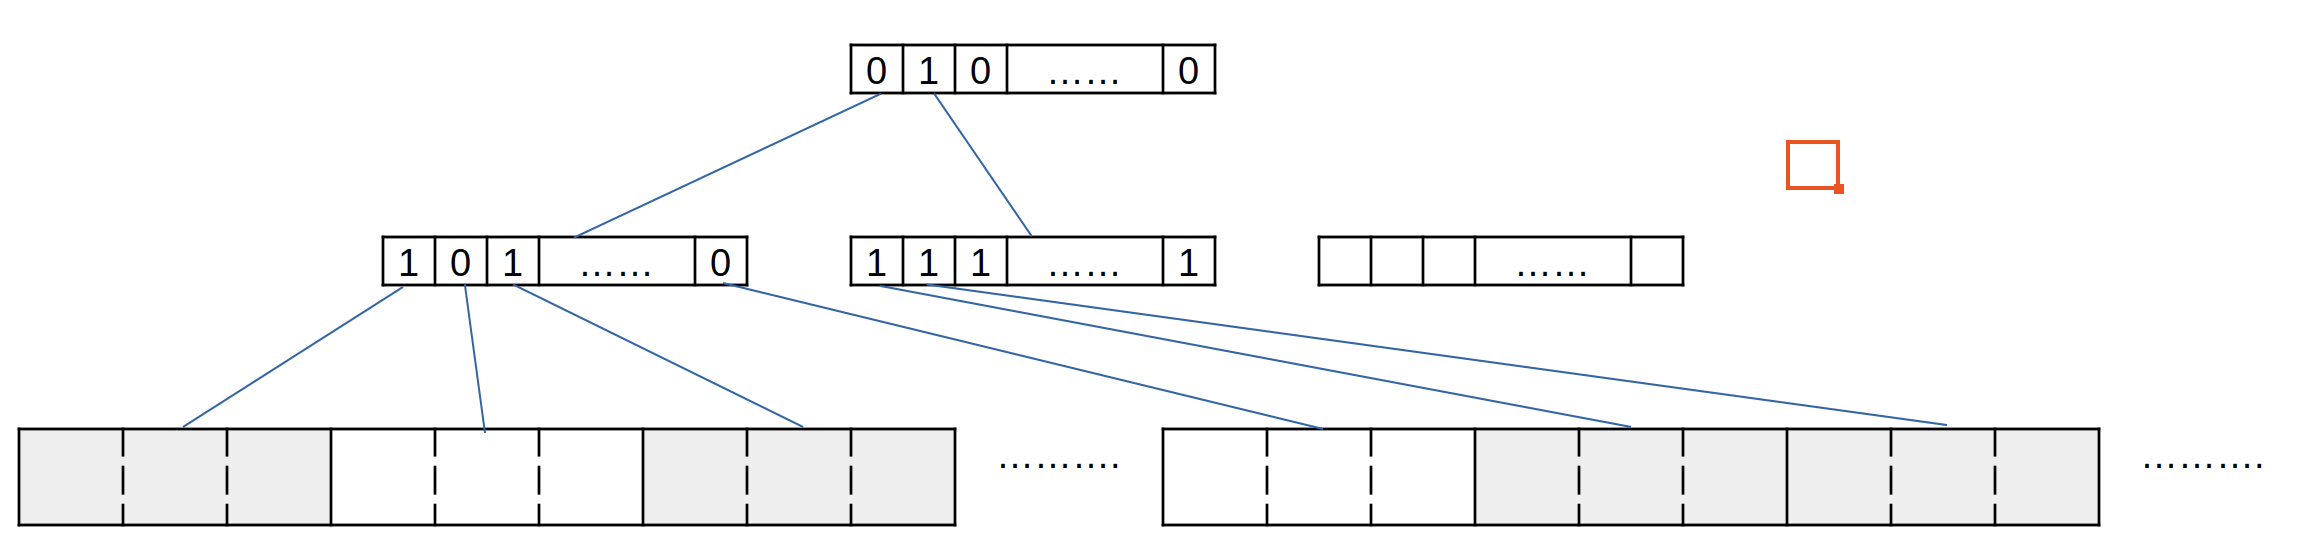
\includegraphics[scale=0.15]{block.png}
		
		\item Сложность выделения или освобождения одного сегмента в блоке -- О(1).
		
		\item Максимальное количество ячеек не попавших ни в один из сегментов (дыра в конце блока) равно 49 
		при размере блока 4096, т.е. примерно 1\%.
		
		\item Размер метаданных одного блока равен 536 байт. Если одна ячейка соответствует 8 байт полезных
		данных, то получается размер метаданных примерно 1.6\% от полезных данных.
	\end{itemize}

	\section{Использование блоков}
	
	\begin{itemize}
		\item Каждый блок может находиться в одном из статусов:
			\begin{enumerate}
				\item Свободный
				\item Частично занят
				\item Полностью занят
			\end{enumerate}
		
		\item Возможные изменения статусов: $1 \leftrightarrow 2 $, $2 \leftrightarrow 3 $.
		
		\item В статусах "Частично занят" и "Полностью занят" блок хранит сегменты одной длины.
		
		\item Все блоки со статусом "Свободный" хранятся в общем списке (двунаправленном).
		
		\item Для каждого допустимого размера сегмента 
		$\textsf{Size} \in \left[ 1,\ldots ,\textsf{MaxBufferSize}\right] $ создается свой список блоков
		со статусом "Частично занят".
		
		\item Блоки при переходе в статус "Полностью занят" удаляются из списка блоков соответствующего размера,
		а при переходе обратно в статус "Частично занят" добавляется в начало списка.
		
	\end{itemize}

	\section{Алгоритм выделения памяти}
	
	\begin{itemize}
		\item Ищем блок в котором будет выделен сегмент:
			\begin{itemize}
				\item Проверяем, если список частично занятых блоков этого размера не пустой,
				то используем первый блок.
				\item Если список свободных блоков не пуст, то используем первый блок. Блок удаляется
				из этого списка и добавляется в список частично занятых блоков этого размера.
				\item Если не удалось найти блок, то возвращаем ошибку.
			\end{itemize}
		
		\item В блоке ищем первую доступную группу, в ней первый свободный сегмент. Возвращаем
		индекс первой ячейки сегмента:
		$$ \textsf{cell\_index} = \textsf{block\_index} \cdot \textsf{BlockSize} + 
		\textsf{segment\_index} \cdot \textsf{Size} $$
	
	\end{itemize}

	\section{Алгоритм освобождения памяти}

	\begin{itemize}
		\item При освобождении передается индекс первой ячейки и размер сегмента. Проверяем, что
		они не выходят за допустимые границы.
		
		\item По индексу ячейки определяем индекс блока и индекс сегмента:
		$$ \textsf{block\_index} = \lfloor \frac{\textsf{cell\_index}}{\textsf{BlockSize}} \rfloor$$
		$$ \textsf{segment\_index} = \frac
			{\textsf{cell\_index} - \textsf{BlockSize} \cdot \textsf{block\_index}}{Size} $$
		
		\item Делаем следующие проверки:
			\begin{itemize}
				 \item В этом блоке хранятся сегменты нужной длины.
				 \item Индекс ячейки правильно восстанавливается по вычисленным значениям.
				 \item Сегмент отмечен как занятый.
			\end{itemize}
		
		\item Отмечаем в блоке сегмент как свободный.
		
		\item Если блок стал пустым, переводим его в статус "Свободный". Если блок до этого "Полностью
		занят", то переводим его в статус "Частично занят" и добавляем в соответствующий размеру список.

	\end{itemize}


\end{document}